\documentclass[11pt]{article}

% --- Packages (kept minimal for portable compilation) ---------------------
\usepackage[utf8]{inputenc}
\usepackage[T1]{fontenc}
\usepackage[margin=1in]{geometry}
\usepackage{amsmath}
\usepackage{amssymb}
\usepackage{booktabs}
\usepackage{enumitem}
\usepackage{verbatim}
\usepackage{xcolor}
\usepackage{graphicx}
\usepackage[hidelinks]{hyperref}

\title{\textbf{Self-Evolving User Interfaces:\\
User Interface evolution with Large Language Models}}

\author{Chandrahas Aroori\\
\small Independent Researcher\\
\small \texttt{chandrahas.aroori@gmail.com}}

\date{June 2026}

\begin{document}
\maketitle

\begin{abstract}
\noindent
Machine learning models are optimized continuously from data, yet the user
interfaces in front of them are hand-authored and frozen at ship time. We argue
this asymmetry can be reduced by treating the interface as an optimizable
artifact. This paper describes \textsc{RecursiveUI}, a system in which an
interface is represented as a typed JSON \emph{layout genome}, runtime events are
recorded in a \emph{routing ledger}, and candidate changes are selected by
replaying logged traces against alternative genomes before they are shipped. The
implemented loop supports reversible layout and routing mutations, records each
change as a hypothesis, and accumulates confirmed move classes into a small
pattern library for later generation. We also argue that durable adaptive
interfaces should be built over applications people already use, treating those
applications as data backends while mutating only the owned front-end. The paper
does not report user-facing outcome results: the representation, ledger, replay
selector, and rollback loop are implemented, but a controlled user study remains
future work. The contribution is a reproducible substrate and control loop for
studying continuously revised interfaces.
\end{abstract}

\section{Introduction}

Agent interfaces increasingly receive heterogeneous output: prose, tool logs,
code diffs, errors, questions, file references, and intermediate reasoning. A
static interface often collapses these into the same surface. The user then
performs the missing routing work manually: opening the diff, resizing the log,
ignoring a stale panel, or correcting the place where an answer should have
appeared.

Those corrections are signal. They show which classes of output needed a
purpose-built home, which panels were starved, and which regions carried more
work than their allocated space. Today that signal is usually discarded because
the interface is ordinary application code: hard to mutate safely, hard to
attribute, and hard to evaluate before exposing a change to a user.

This paper narrows self-evolving interfaces to a tractable first problem: can an
interface learn, from its own routing traces, where different classes of output
should live? \textsc{RecursiveUI} answers this with three mechanisms. A typed JSON
\emph{layout genome} makes interface changes discrete and diffable. A
\emph{routing ledger} records what data arrived and where the interface placed
it. A replay-gated evolution loop tests candidate genomes against recorded
sessions, ships only bounded changes, and rolls them back when the measured fit
does not hold.

This does not solve all of interface quality. The current loop optimizes
information placement, not typography, aesthetics, or interaction feel. It also
does not require a freshly generated interface for every task. Generation is a
bootstrap step; the durable target is an owned front-end that can keep improving
over repeated use. In the longer-term substrate we argue for, that front-end sits
over applications a person already uses, treating them as data backends while the
owned interface evolves.

\paragraph{Contributions.}
\begin{enumerate}[leftmargin=1.4em,itemsep=2pt]
  \item A representation (\S\ref{sec:genome}): the \emph{layout genome}, a typed
  JSON intermediate representation of an interface in which mutation is discrete,
  telemetry attaches to stable slot identifiers, and a candidate can be scored
  offline against recorded sessions.
  \item A data plane (\S\ref{sec:loop}): the \emph{routing ledger}, which records
  each event's payload class, destination, and outcome so interface fit can be
  measured from ordinary use.
  \item A control loop (\S\ref{sec:loop}): deterministic morphs and model-proposed
  routing changes are selected by trace replay, shipped as reversible hypotheses,
  and summarized in a shared pattern library.
  \item A set of design constraints (\S\ref{sec:position}): self-evolving
  interfaces need durable use, an owned mutation boundary, and stable data access.
  \item An evaluation boundary (\S\ref{sec:eval}, \S\ref{sec:limits}): what the
  offline metric measures, what it does not measure, and the online protocol a
  controlled study would require.
\end{enumerate}

We describe a system, \textsc{RecursiveUI}, that implements points 1--3. It is a
desktop application that hosts purpose-built interfaces for AI agent skills; the
implementation is the existence proof for the representation and the loop, not a
product claim. Source is available.\footnote{\url{https://github.com/Exorust/RecursiveUI}}
Figure~\ref{fig:loop} shows the whole system as a single closed loop.

\begin{figure}[t]
\centering
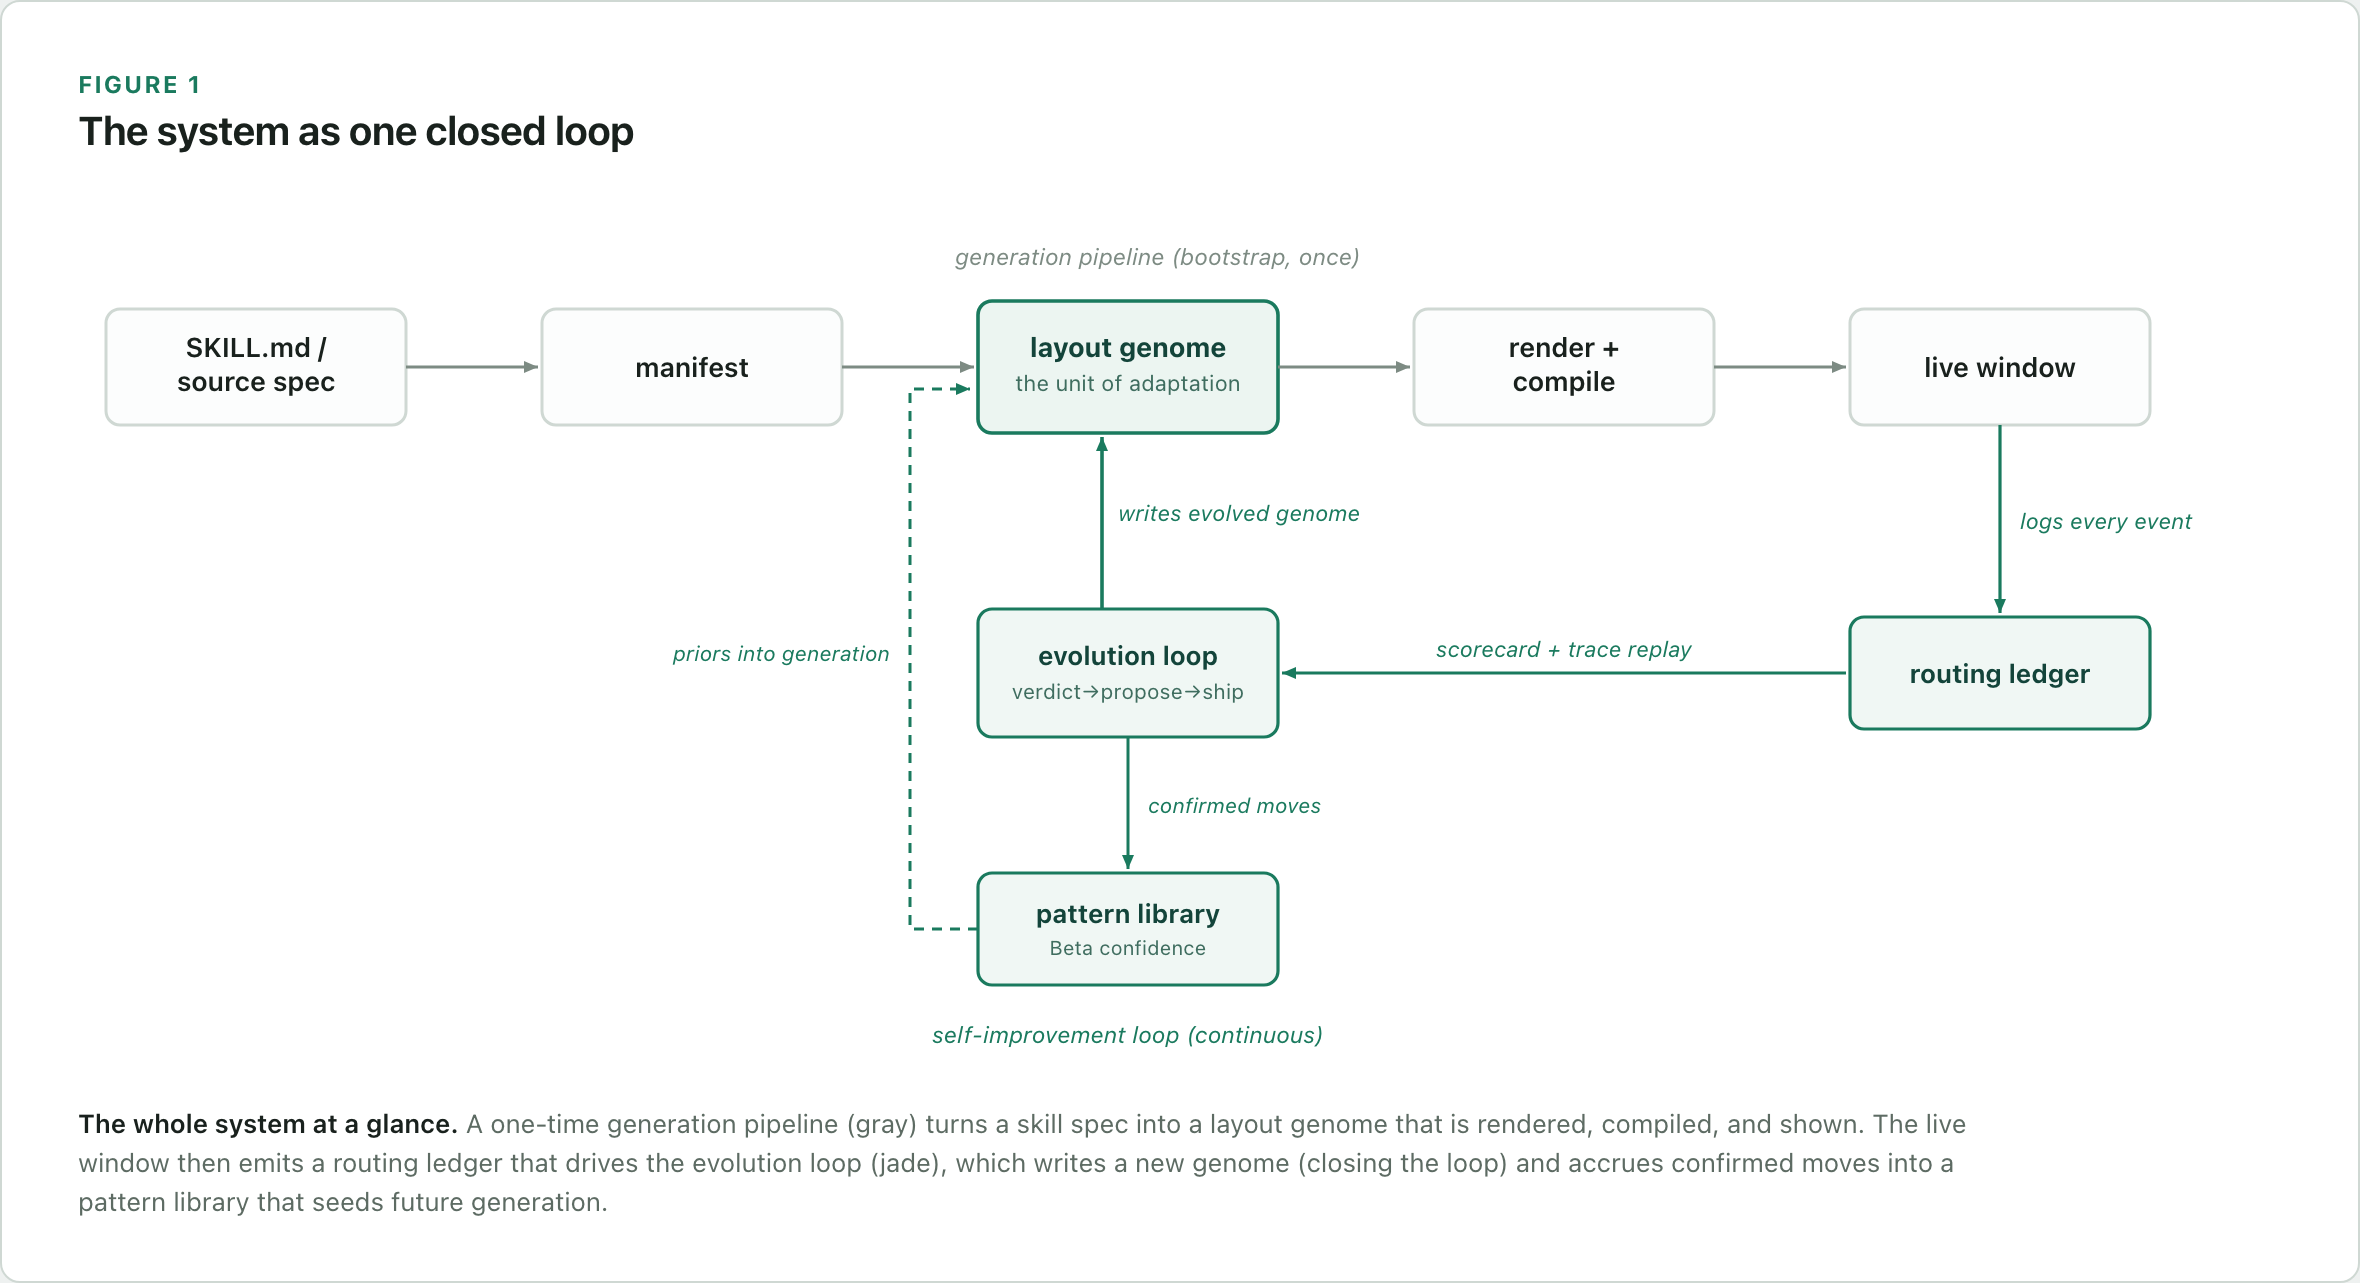
\includegraphics[width=\textwidth]{figures/fig1.png}
\caption{The system as one closed loop. A one-time generation pipeline (gray)
turns a skill specification into a layout genome that is rendered, compiled, and
shown. The live window emits a routing ledger that drives the evolution loop
(jade), which writes a new genome (closing the loop) and accrues confirmed moves
into a pattern library that seeds future generation.}
\label{fig:loop}
\end{figure}

\section{Background and Related Work}
\label{sec:related}

\paragraph{Adaptive and self-optimizing interfaces.}
The idea that an interface should reorganize around use is old and well studied.
Sears and Shneiderman's split menus moved frequently selected items to the top of
a menu and reduced selection time by 17--47\% in controlled and field
studies~\cite{sears1994split}. The literature since has mapped the space of
\emph{adaptive} (system-driven), \emph{adaptable} (user-driven), and static
interfaces, and is careful about the costs of adaptation: Findlater and
McGrenere found that poorly predicted adaptation can be slower than no adaptation
at all~\cite{findlater2004comparison}, and Gajos et al.\ charted the design
dimensions that determine whether an adaptive GUI helps or
hurts~\cite{gajos2006design}. \textsc{Supple} reframed interface generation as
optimization over a large discrete space and showed it is tractable and that the
generated interfaces measurably outperform manufacturer defaults for users with
motor impairments~\cite{gajos2010supple}. Our work inherits directly from
this line. The differences are mechanical and consequential: our optimization
target is derived automatically and continuously from a usage ledger rather than
from an explicit cost model or a one-time study, the representation under
optimization is a recursive component layout rather than a widget tree, and a
language model is admitted as one proposal mechanism among deterministic ones,
gated by an offline evaluator.

\paragraph{Generating interfaces and code with models.}
Generating UI from higher-level signals predates large language models;
\textsc{pix2code} produced markup from a screenshot~\cite{beltramelli2017pix2code}.
Code-trained language models made free-form UI generation easy and now
commonplace~\cite{chen2021codex}. We treat generation as necessary plumbing, not
as the product. The failure mode we want to avoid is precisely the one that
generation makes tempting: producing a bespoke interface per task that is
impressive once and then has no reason to be reopened. Generation in our system
stands up the first version of a front-end; the contribution is what happens to
that front-end afterward.

\paragraph{Self-improving agents and skill libraries.}
A parallel and recent line lets agents improve their own \emph{capabilities}.
\textsc{Voyager} maintains an ever-growing library of executable skills, written
and refined by a language model against environment feedback, and reuses it
across tasks~\cite{wang2023voyager}. Generative agents accumulate and retrieve
memory to drive consistent behavior over time~\cite{park2023generative}. In
production, NousResearch's Hermes Agent ships a closed learning loop that writes
skills from experience and runs a periodic curator to score, merge, and prune the
skill library, exposed through a single durable operations
dashboard~\cite{hermes2026}. These systems adapt agent behavior or skill choice.
\textsc{RecursiveUI} instead treats the interface layout and routing policy as
the object under revision. Hermes' use of one durable dashboard is consistent
with the argument in \S\ref{sec:seenonce}, but our claim does not depend on it.

\paragraph{Learning from interaction: bandits, preferences, and offline
evaluation.}
The machinery for optimizing a decision from logged behavior is mature.
Contextual bandits select among options to maximize a reward signal estimated
from interaction~\cite{li2010contextual}, with Thompson sampling a standard
strategy for balancing exploration and exploitation~\cite{thompson1933,chapelle2011thompson}.
Reinforcement learning from human preferences turns pairwise judgments into an
optimization signal~\cite{christiano2017preferences,ouyang2022instructgpt}, and
counterfactual / offline policy evaluation estimates how an unshipped policy
would have performed on logged data~\cite{bottou2013counterfactual}. Our loop is
an applied, conservative instance of these ideas: the Beta-confidence pattern
library is a per-move-class Bernoulli posterior, the trace-replay selector is a
narrow form of offline evaluation specialized to interface routing, and the
hypothesis register with automatic rollback is online experimentation with a
safety bias toward the incumbent.

\section{Design Constraints for Self-Evolving Interfaces}
\label{sec:position}

\subsection{Why single-use generation is the wrong target}
\label{sec:seenonce}

The most direct way to apply a language model to interface construction is to
generate a UI for each task on demand. We built an early version of this and
found that it produced the wrong optimization problem. A surface that is seen
once has no longitudinal trace, no stable user investment, and no meaningful
before/after comparison. It can be impressive as generation, but it gives the
system little evidence for improvement.

The target must instead be a durable interface: one that is opened repeatedly,
serves related work over time, and accumulates routing mistakes that can be
measured. This changes the role of generation. The model can create an initial
genome, but the research problem is what happens after that genome has handled
real sessions. A self-evolving interface needs history more than novelty.

\subsection{The ownership boundary}
\label{sec:appsasbackends}

The second constraint is control. An evolution loop cannot safely mutate an
interface it does not own. Host application markup changes, class names are not a
contract, and direct DOM edits compete with the host renderer. The boundary used
in this paper is therefore simple: mutate only the owned front-end, and treat
external applications or agent runtimes as data sources.

\textsc{RecursiveUI} currently implements this boundary for owned agent-skill
interfaces. The system controls the layout, routing table, component catalog, and
version history; the agent supplies events. The broader
applications-as-backends framing uses the same boundary. An existing application
is valuable because it already contains the user's data and workflow, but the
adaptive surface should be a front-end rendered over that data, not a patch
against the host application's private UI.

\paragraph{The stability ladder.}
When the data source is an existing application, the front-end should read from
the most stable available contract, in order:
\begin{enumerate}[leftmargin=1.6em,itemsep=1pt]
  \item \textbf{Official API.} Structured, versioned, intended for programmatic
  use.
  \item \textbf{Accessibility roles.} ARIA roles and labels (or a native
  accessibility tree), which are more semantic than visual class names.
  \item \textbf{URL / deep links.} Many applications expose navigable state in
  their address.
  \item \textbf{DOM scraping.} A last resort, assumed brittle and isolated behind
  repair logic.
\end{enumerate}

\subsection{What this implies for the representation}

These constraints determine the architecture that follows. Durability requires
stable identifiers so telemetry can survive across versions. The ownership
boundary requires a representation that can be mutated without executing
arbitrary host code. Offline selection requires changes that can be replayed
against prior events. The layout genome in the next section is the result: a
small, typed intermediate representation where layout, slots, routing, tokens,
and provenance are explicit data rather than opaque application code.

\section{The Layout Genome}
\label{sec:genome}

The unit of adaptation is a typed JSON document we call a \emph{layout genome}. A
rendered interface is a \emph{function of} the genome, not the source of truth.
This indirection is what makes adaptation safe and measurable: mutations are
discrete and diffable, telemetry attaches to stable slot identifiers across
versions, and a candidate genome can be scored offline against recorded sessions
(\S\ref{sec:loop}).

A genome has four parts.

\begin{itemize}[leftmargin=1.4em,itemsep=2pt]
  \item A recursive \textbf{layout tree} of containers
  (\texttt{split-h}, \texttt{split-v}, \texttt{stack}, \texttt{tabs},
  \texttt{grid}) whose leaves reference slots, with per-child size weights. This
  is the structure, in the spirit of tiling window managers and auto-layout.
  \item A \textbf{slot} table mapping each leaf identifier to a catalog component,
  a semantic \texttt{role} (a WAI-ARIA-flavored label that is also a stable
  routing target), typed \texttt{params} (the surface the deterministic tuner
  acts on), optional presentation \texttt{conditions}, and an \texttt{evolvable}
  flag that fences hand-authored or locked slots off from the automatic loop.
  \item A \textbf{routing} table: ordered \texttt{match$\rightarrow$slot} rules
  (matching on event type, a payload class, or a tool name, first match wins)
  with exactly one terminal \texttt{fallback} sink. Routing is the data plane: it
  decides where each incoming event is shown.
  \item \textbf{Tokens} (accent, density) and \textbf{provenance}: the source of
  the genome (\texttt{generated}, \texttt{evolved}, \texttt{studio},
  \texttt{community}) and a \texttt{parentHash} that anchors each change to the
  version it was derived from.
\end{itemize}

A compact example, lightly abridged; Figure~\ref{fig:genome} shows the same
genome beside the interface it renders:

\begin{footnotesize}
\begin{verbatim}
{
  "skill": "code-review", "source": "generated",
  "tokens": { "accent": "jade", "density": "comfortable" },
  "tree": { "type": "split-h", "sizes": [32, 68], "children": [
      { "slot": "chat" },
      { "type": "split-v", "sizes": [66, 34],
        "children": [ { "slot": "diff" }, { "slot": "findings" } ] } ] },
  "slots": {
    "chat":     { "component": "AgentChat", "role": "main", "evolvable": true },
    "diff":     { "component": "DiffViewer", "role": "complementary",
                  "params": { "mode": "unified" } },
    "findings": { "component": "FindingsPanel", "role": "log" } },
  "routing": [
    { "match": { "payloadClass": "diff" },        "to": "diff" },
    { "match": { "event": "tool_execution_*" },   "to": "findings" },
    { "match": { "payloadClass": "text" },        "to": "chat" },
    { "fallback": "chat" } ]
}
\end{verbatim}
\end{footnotesize}

\begin{figure}[t]
\centering
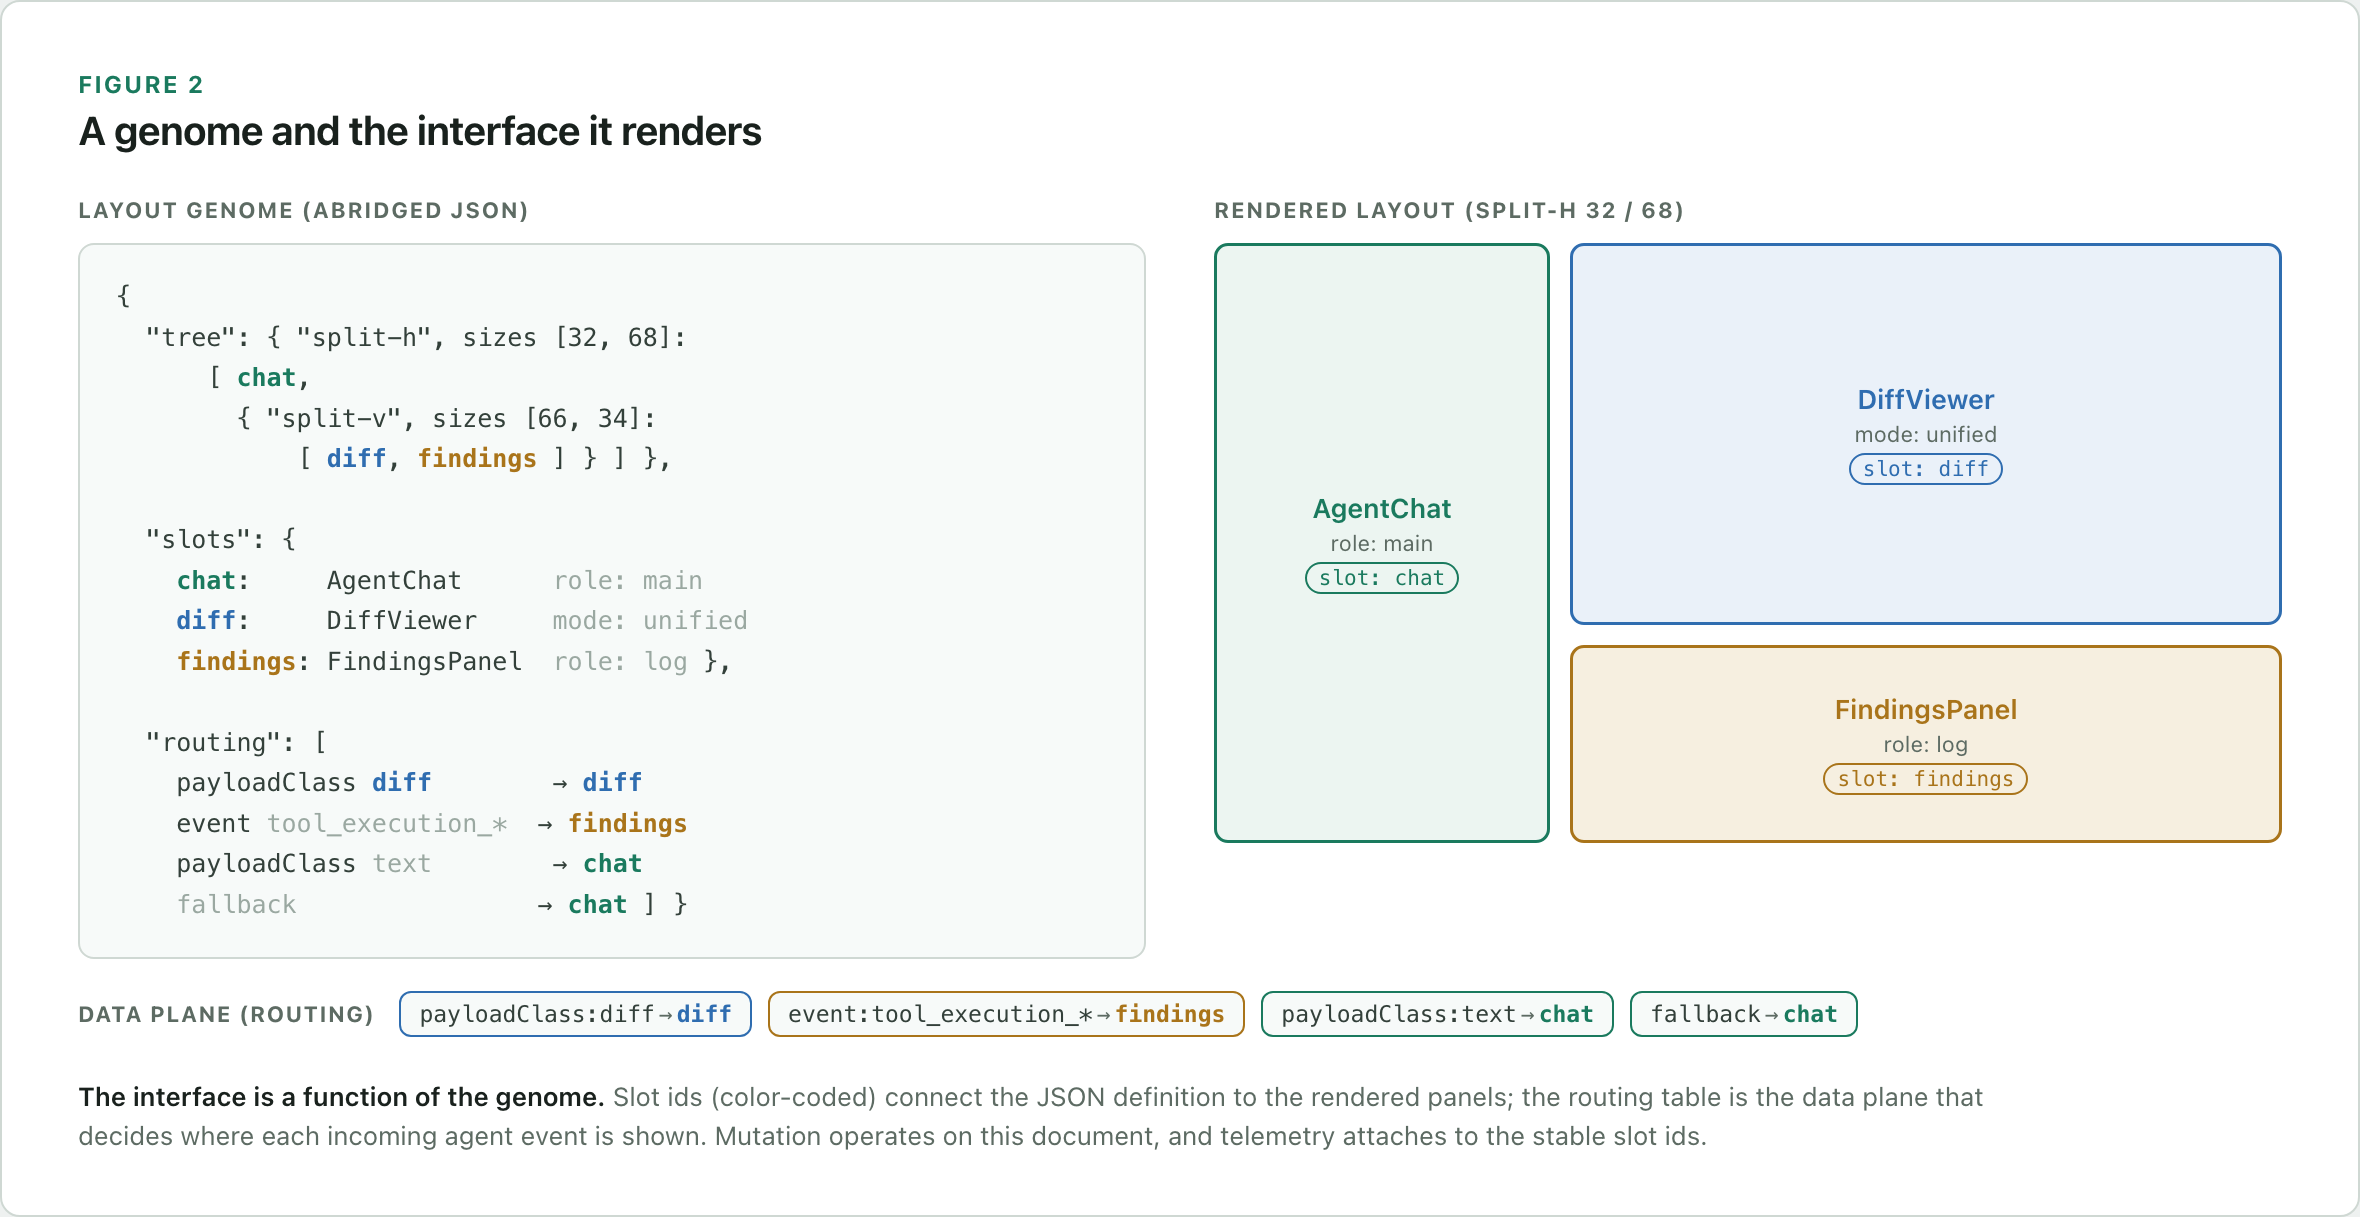
\includegraphics[width=\textwidth]{figures/fig2.png}
\caption{A layout genome and the interface it renders. Color-coded slot ids link
the JSON definition to the rendered panels; the routing table is the data plane
that decides where each incoming agent event is shown. Mutation operates on this
document, and telemetry attaches to the stable slot ids.}
\label{fig:genome}
\end{figure}

The genome is validated before anything renders (every routing target must name a
real slot; exactly one fallback must exist), then deterministically rendered to
component code and compiled. Generated code is import-free and binds to the
component catalog through a host-provided kit, so a genome can be authored or
mutated without the renderer trusting arbitrary imports. In the
applications-as-backends framing of \S\ref{sec:appsasbackends}, the catalog
components are the owned front-end and a slot's routing source is the host
application's data feed; the representation is unchanged.

\paragraph{Implementation status.}
In the current implementation, genomes are stored as versioned JSON records with
a parent hash, and each accepted mutation creates a new version rather than
rewriting the old one. Ledger records are appended during live sessions as agent
events pass through the router. Evolution is triggered after enough new ledger
records have accumulated for an interface; the current thresholds for minimum
sessions, fit improvement, and rollback are fixed configuration values rather
than learned parameters. This makes the loop reproducible, but it also means the
policy is still a hand-engineered controller.

\paragraph{Generation as bootstrapping.}
The first genome for a new interface is produced by a pipeline that parses the
task's specification into a manifest, prompts a model for a genome (seeded with
patterns previously confirmed on \emph{other} interfaces; see
\S\ref{sec:patterns}), validates, renders, compiles, and commits the result to a
per-interface version history. Generation is deliberately confined to this
bootstrap. Everything after it is the loop.

\section{The Routing Ledger and the Evolution Loop}
\label{sec:loop}

\subsection{The routing ledger}

The signal that drives adaptation is a log that records two things together: what
data arrived, and what the interface did with it. Every agent event is classified
into a \emph{payload class} (for example \texttt{diff}, \texttt{tool\_output},
\texttt{thinking}, \texttt{text}, \texttt{question}) and resolved against the
genome's routing into one of three outcomes: \texttt{routed} (it found a
purpose-built slot), \texttt{fallback} (it was shown, but only in the default
sink), or \texttt{dropped} (no home at all). Each record carries the event type,
the payload class, a byte size as a coarse magnitude, the resolved slot, and the
outcome.

Because the system owns both routing and layout, each event can be logged with
its payload class, destination, and outcome. This produces the supervision signal
used by the evolution loop without requiring separate instrumentation from the
interface author.

\subsection{The scorecard}

From the ledger we derive, in pure queries, a per-interface scorecard. The
central quantity is the \emph{fit score}, the fraction of output (by bytes) that
was routed to a real slot rather than to the fallback or dropped:
\[
  \mathrm{fit} = \frac{\text{routed bytes}}{\text{routed} + \text{fallback} + \text{dropped bytes}}.
\]
The scorecard also reports, per payload class, how much is chronically falling
back (a class with no home), and, per slot, how busy or starved it is (the share
of routed output it carries, and whether it has received anything at all). These
three views map directly to the three morphs below.

\subsection{The cycle}

A cycle runs in four phases: \textsc{verdict}, \textsc{diagnose},
\textsc{propose}, \textsc{ship}.

\paragraph{Verdict.} If a previous change is live, the cycle first judges it.
After a minimum number of sessions have accumulated under the change, if fit has
held at or above a threshold the change is \emph{confirmed}; otherwise it is
\emph{reverted} to its parent genome and the move class is placed on cooldown.
Either way the outcome updates the pattern library (\S\ref{sec:patterns}). This
phase is what makes the loop safe to run unattended: a change that does not pay
for itself is automatically rolled back.

\paragraph{Diagnose and propose.} The system proposes at most one change, trying
mechanisms in order of cost and reversibility:
\begin{enumerate}[leftmargin=1.6em,itemsep=2pt]
  \item \textbf{Resize} (deterministic). If one slot carries a dominant share of
  routed output but holds a minority of the space, grow it. A pure,
  reversible, one-field edit driven entirely by the ledger. This is the analogue,
  for a recursive layout, of moving frequent items up a split menu.
  Figure~\ref{fig:morph} shows a before/after.
  \item \textbf{Prune} (deterministic). If a slot mounted in the tree has
  received no routed output across the observed sessions, remove it and reclaim
  its space; never the fallback sink.
  \item \textbf{Fallback fix} (model-proposed, evaluator-gated). If a payload
  class is chronically hitting the fallback, there is no component receiving it.
  Only here is a language model invoked, and only to \emph{propose}: it is asked
  to add or re-route a slot so that class lands somewhere purposeful.
\end{enumerate}
Deterministic morphs are preferred not for taste but because they are cheap,
reversible, and need no evaluation to trust. The model is reserved for the one
case the data poses but cannot itself answer: a recurring need with no home.

\begin{table}[t]
\centering
\begin{tabular}{p{0.17\linewidth}p{0.27\linewidth}p{0.27\linewidth}p{0.18\linewidth}}
\toprule
Move & Trigger & Mutation & Gate \\
\midrule
Resize & Busy slot, small region & Change split weights & Hypothesis verdict \\
Prune & Mounted slot receives no routed output & Remove slot from tree & Hypothesis verdict \\
Fallback fix & Payload class repeatedly falls back & Add or reroute slot & Trace replay \\
\bottomrule
\end{tabular}
\caption{Implemented move classes. Deterministic moves are still shipped under a
rollback hypothesis; model-proposed routing changes must also beat the incumbent
under offline replay before shipping.}
\label{tab:morphs}
\end{table}

\begin{figure}[t]
\centering
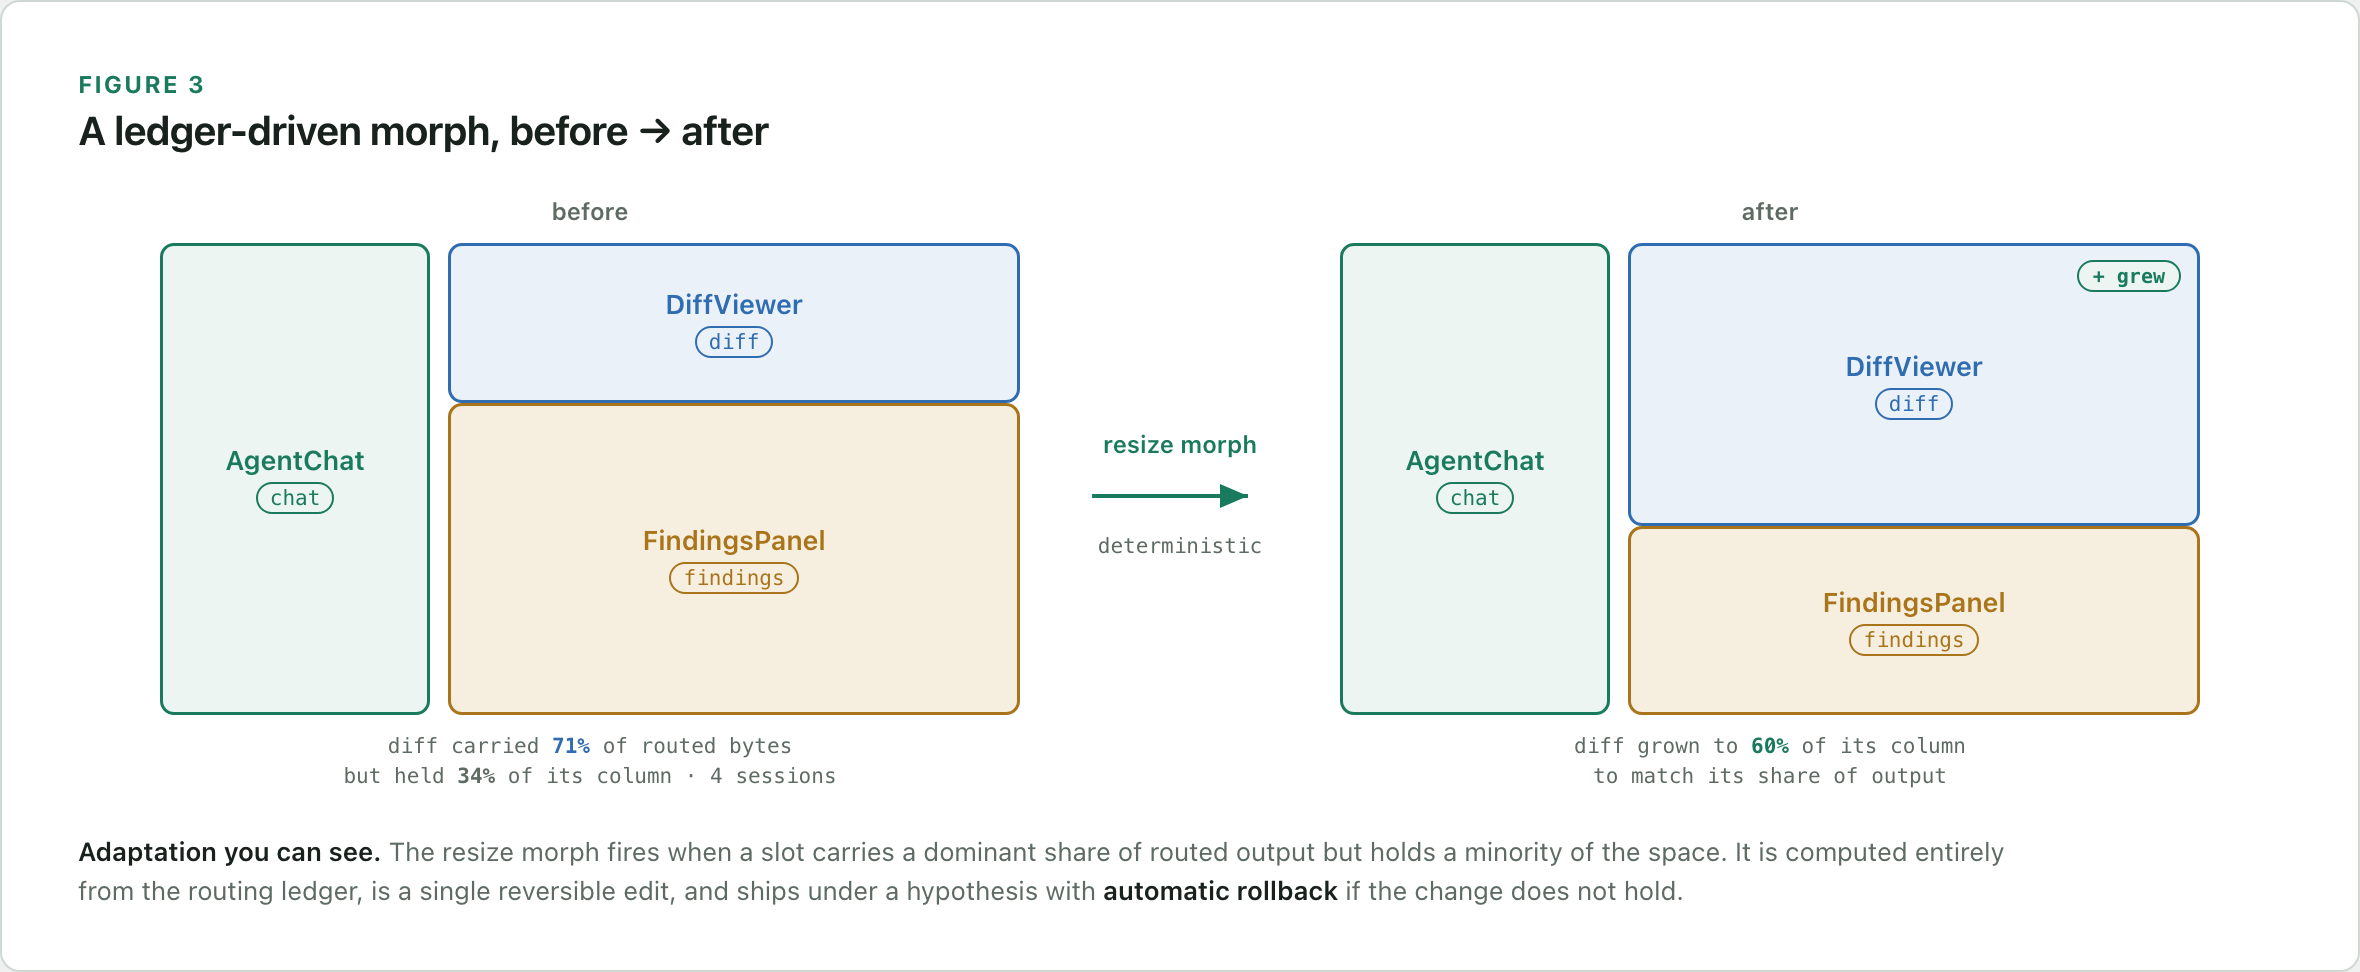
\includegraphics[width=\textwidth]{figures/fig3.png}
\caption{A ledger-driven resize morph, before and after. The morph fires when a
slot carries a dominant share of routed output (here the diff pane, 71\% of bytes)
but holds a minority of the space (34\%); it grows the pane to match. The change
is a single reversible edit, computed from the routing ledger and shipped under a
hypothesis with automatic rollback.}
\label{fig:morph}
\end{figure}

\paragraph{Trace replay selection.} A model proposal is not shipped directly.
Each candidate genome is scored by \emph{trace replay}: the recorded events are
re-routed through the candidate's routing table, and its fit is recomputed as if
it had been live during those sessions. The candidate ships only if its replayed
fit beats the incumbent by a margin. This is offline policy evaluation narrowed
to interface routing: replay can score a change to \emph{where data goes}; it
cannot score a purely visual or interaction change, because the ledger does not
encode aesthetics. Replay is therefore a gate on routing mutations, not a
universal fitness function.

\paragraph{Ship under hypothesis.} A surviving change is committed as a new
genome version and recorded in a \emph{hypothesis register}: the move class, the
diff, the human-readable rationale, the predicted metric and direction, and,
critically, the full parent genome, so the \textsc{verdict} phase can revert it
exactly. Each change is therefore stored with both its expected effect and its
rollback condition.

\subsection{The pattern library: turning outcomes into priors}
\label{sec:patterns}

Each move class (resize, prune, fallback-fix, and finer-grained future variants)
carries a Beta--Bernoulli confidence: confirmed and refuted counts summarized by
the posterior mean $(\text{confirms}+1)/(\text{confirms}+\text{refutes}+2)$. Two
things follow. Confidence is shared across all interfaces, so a move that
repeatedly pays off anywhere accrues evidence everywhere, and one that repeatedly
fails stops being tried. And move classes that clear a confidence threshold are
injected as \emph{priors into generation}: the bootstrap prompt for a new
interface is seeded with the layout moves that have been confirmed on others. The
loop thereby improves not only individual interfaces but the starting point of
every future one. This is the cross-context transfer that distinguishes a library
of adaptations from per-interface tuning.

\section{Current Evaluation and Study Protocol}
\label{sec:eval}

The representation, ledger, scorecard, evolution loop, trace-replay selector, and
pattern library are implemented. The current evaluation is best understood as
regression control for routing changes, not evidence of improved usability. We
therefore separate the internal checks the system runs today from the controlled
study needed to measure user outcomes.

\paragraph{Implemented internal checks.}
The fit score and its decomposition are computed continuously from the ledger,
and trace replay scores candidate genomes against recorded sessions. These are
internal selection signals, and their validity is bounded: fit is a proxy
(``did output find a purpose-built home?''), bytes are a coarse stand-in for
attention, and replay is blind to anything that is not a routing decision. They
are appropriate as a conservative gate on shipping routing changes and
inappropriate as a claim about user outcomes.

\paragraph{The online protocol a real study needs.}
To test whether self-evolution helps users, the hypothesis register already
provides the experimental scaffold; what is missing is a controlled deployment
and outcome metrics. The protocol we would run:
\begin{itemize}[leftmargin=1.4em,itemsep=1pt]
  \item \textbf{Design.} Within-subjects across tasks, comparing the frozen
  bootstrap genome against the evolved genome, with the hypothesis register's
  automatic rollback providing safe single-change A/B units.
  \item \textbf{Outcome metrics.} Time to task completion; correction rate (how
  often the user reorganizes or overrides the interface); fit as a secondary,
  process metric; task success/completion.
  \item \textbf{Preference labels.} Pairwise keep/revert judgments at change
  boundaries, yielding gold labels for the pattern library in the style of
  preference learning~\cite{christiano2017preferences}.
  \item \textbf{Analysis.} Whether evolved interfaces reduce time and corrections
  over sessions relative to the frozen control, and whether confirmed patterns
  transfer to held-out interfaces (measured as bootstrap fit on interfaces the
  pattern was not derived from).
\end{itemize}

\section{Limitations and Threats to Validity}
\label{sec:limits}

\begin{itemize}[leftmargin=1.4em,itemsep=2pt]
  \item \textbf{Cold start.} Adaptation needs accumulated sessions before it acts.
  The bootstrap genome and the cross-interface pattern priors mitigate this but do
  not remove it; the first sessions are unadapted by construction.
  \item \textbf{Proxy metrics.} Bytes approximate attention badly (a small,
  critical error message and a verbose log are weighted by size), and the fit
  threshold and replay margin are hand-set heuristics, not learned.
  \item \textbf{Single-user adaptation.} The loop optimizes for the observed user.
  Whether this is a feature (a personal tool) or a risk (overfitting, a UI that
  drifts away from any shareable norm) is unresolved and depends on deployment.
  \item \textbf{Model proposals.} The one model-driven morph inherits the cost,
  latency, and nondeterminism of a language model; the evaluator gate contains but
  does not eliminate the risk of a plausible-looking but worse proposal.
  \item \textbf{The applications-as-backends regime is not yet evaluated.}
  The stability ladder and substrate argument (\S\ref{sec:appsasbackends}) define
  an intended deployment boundary, not yet an evaluated subsystem of
  \textsc{RecursiveUI}. Re-fronting an application incurs real per-application
  work, and raw automation inherits the reliability problems of computer use.
\end{itemize}

\section{Open Problems}
\label{sec:open}

The current system leaves several research problems open.
\begin{enumerate}[leftmargin=1.5em,itemsep=2pt]
  \item \textbf{Evaluating interface quality beyond routing.} Fit measures
  whether data reached a purpose-built slot. It does not measure spacing,
  typography, motion, interaction cost, or whether the user preferred the result.
  \item \textbf{Credit assignment over time.} When a session goes well, which of
  several recent interface changes deserves credit? The current one-live-change
  discipline sidesteps the problem rather than solving it.
  \item \textbf{Personal versus shared interfaces.} How should a single library of
  patterns serve both a UI that overfits to one expert and a UI that must stay
  legible to a newcomer?
  \item \textbf{Safety of self-modifying interfaces.} Auto-rollback bounds harm,
  but what are the right invariants a self-evolving interface must never violate
  (accessibility, discoverability, destructive-action friction)?
  \item \textbf{A benchmark.} The field has no shared benchmark for self-evolving
  interfaces: a corpus of tasks, recorded interaction traces, and a scoring
  harness against which different loops could be compared. Trace replay is a
  starting primitive for one.
  \item \textbf{Substrate adaptation.} Combining the accessibility-tree substrate
  with the evolution loop, so that an owned front-end over an arbitrary host
  application adapts from observed use, is the concrete next system.
\end{enumerate}

\section{Conclusion}

\textsc{RecursiveUI} shows that interface adaptation can be made concrete by
moving from opaque UI code to a typed layout genome, from unstructured usage to a
routing ledger, and from direct model edits to replay-gated, reversible
mutations. The implemented system establishes this substrate and control loop for
owned agent-skill interfaces. It does not yet establish that evolved interfaces
improve user outcomes; that requires the controlled study described above.

\section*{Reproducibility}
The representation, generation pipeline, routing ledger, scorecard, evolution
loop, trace-replay selector, and pattern library described here are implemented
and openly available at \url{https://github.com/Exorust/RecursiveUI}. No
human-subjects data is reported and none was
collected; all internal metrics are derived from the system's own routing ledger.

\begin{thebibliography}{99}
\setlength{\itemsep}{2pt}

\bibitem{sears1994split}
A.~Sears and B.~Shneiderman.
\newblock Split menus: effectively using selection frequency to organize menus.
\newblock \emph{ACM Transactions on Computer-Human Interaction}, 1(1):27--51, 1994.

\bibitem{findlater2004comparison}
L.~Findlater and J.~McGrenere.
\newblock A comparison of static, adaptive, and adaptable menus.
\newblock In \emph{Proc. CHI}, 2004.

\bibitem{gajos2006design}
K.~Z. Gajos, M.~Czerwinski, D.~S. Tan, and D.~S. Weld.
\newblock Exploring the design space for adaptive graphical user interfaces.
\newblock In \emph{Proc. AVI}, 2006.

\bibitem{gajos2010supple}
K.~Z. Gajos, D.~S. Weld, and J.~O. Wobbrock.
\newblock Automatically generating personalized user interfaces with Supple.
\newblock \emph{Artificial Intelligence}, 174(12--13):910--950, 2010.

\bibitem{beltramelli2017pix2code}
T.~Beltramelli.
\newblock pix2code: Generating code from a graphical user interface screenshot.
\newblock \emph{arXiv:1705.07962}, 2017.

\bibitem{chen2021codex}
M.~Chen et al.
\newblock Evaluating large language models trained on code.
\newblock \emph{arXiv:2107.03374}, 2021.

\bibitem{wang2023voyager}
G.~Wang, Y.~Xie, Y.~Jiang, A.~Mandlekar, C.~Xiao, Y.~Zhu, L.~Fan, and A.~Anandkumar.
\newblock Voyager: An open-ended embodied agent with large language models.
\newblock \emph{arXiv:2305.16291}, 2023.

\bibitem{park2023generative}
J.~S. Park, J.~C. O'Brien, C.~J. Cai, M.~R. Morris, P.~Liang, and M.~S. Bernstein.
\newblock Generative agents: Interactive simulacra of human behavior.
\newblock In \emph{Proc. UIST}, 2023.

\bibitem{li2010contextual}
L.~Li, W.~Chu, J.~Langford, and R.~E. Schapire.
\newblock A contextual-bandit approach to personalized news article recommendation.
\newblock In \emph{Proc. WWW}, 2010.

\bibitem{thompson1933}
W.~R. Thompson.
\newblock On the likelihood that one unknown probability exceeds another in view of the evidence of two samples.
\newblock \emph{Biometrika}, 25(3/4):285--294, 1933.

\bibitem{chapelle2011thompson}
O.~Chapelle and L.~Li.
\newblock An empirical evaluation of Thompson sampling.
\newblock In \emph{Advances in Neural Information Processing Systems (NeurIPS)}, 2011.

\bibitem{christiano2017preferences}
P.~Christiano, J.~Leike, T.~B. Brown, M.~Martic, S.~Legg, and D.~Amodei.
\newblock Deep reinforcement learning from human preferences.
\newblock In \emph{Advances in Neural Information Processing Systems (NeurIPS)}, 2017.

\bibitem{ouyang2022instructgpt}
L.~Ouyang et al.
\newblock Training language models to follow instructions with human feedback.
\newblock In \emph{Advances in Neural Information Processing Systems (NeurIPS)}, 2022.

\bibitem{bottou2013counterfactual}
L.~Bottou, J.~Peters, J.~Qui\~{n}onero-Candela, D.~X. Charles, D.~M. Chickering,
E.~Portugaly, D.~Ray, P.~Simard, and E.~Snelson.
\newblock Counterfactual reasoning and learning systems: The example of computational advertising.
\newblock \emph{Journal of Machine Learning Research}, 14:3207--3260, 2013.

\bibitem{hermes2026}
NousResearch.
\newblock Hermes Agent (software).
\newblock \url{https://github.com/nousresearch/hermes-agent}, accessed 2026.

\end{thebibliography}

\end{document}
